%!TEX root = ../dokumentation.tex
\chapter{Grundlagen Elektronik}\label{chapter:grundlagenet}
\section{Photodioden}\label{sec:photodioden}
Um Licht zu detektieren werden meist Photodioden verwendet. Diese arbeiten nach einem relativ einfachen Prinzip.
Eine p-n-Diode wird in Sperrrichtung betrieben, durch die Angelegte Spannung entsteht eine Sperrschicht. Wenn nun Photonen auf die offene, starke p-Dotierung treffen werden dort durch den Photoeffekt Ladungsträger erzeugt (Abbildung: \ref{photodiode}). Wenn diese nun durch Diffusion bis zur Sperrschicht gelangen, driften die Ladungsträger entgegen der Sperrspannung in die jeweiligen Raumladungszonen, dies ist als Strom messbar. \cite{Photodiode_spektrum}
\begin{figure}[H]
	\centering
	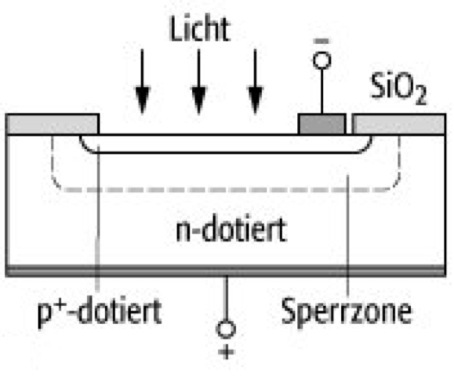
\includegraphics[width=0.75\textwidth]{images/GrundlagenLaserentfernungsmessung/Photodiode}
	\caption{Schematischer Aufbau einer Photodiode \cite{Photodiode_spektrum} ($p^+$ starke p-Dotierung)}
	\label{photodiode}
\end{figure}
Dieser Effekt tritt allerdings nur auf, wenn die Photonen eine Energie großer als die des Bandabstandes des verwendeten Halbleiters aufweisen. Hierbei ist zudem pro eintreffendem Photon nur ein sehr geringer Stromimpuls messbar, daher ist diese Art von Diode für \ac{LIDAR} Anwendungen nicht brauchbar.
\subsection{\acf{APD}}\label{subsec:apd}
Um einzelne Photonen detektieren zu können wird eine spezielle Form der Photodiode verwendet. Die sogenannte \ac{APD}. Die \ac{APD} hat im Gegensatz zur herkömmlichen Photodiode zweit weitere Schichten. Hinzu zur n-Dotierten und stark p-Dotierten Schicht kommen nun eine schwach p-Dotierte (oder intrinsische) und eine "normal" p-Dotierte Schicht (Abbildung: \ref{apd}). 
\begin{figure}[H]
	\centering
	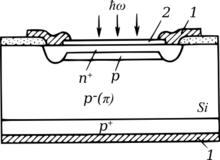
\includegraphics[width=0.75\textwidth]{images/GrundlagenLaserentfernungsmessung/APD}
	\caption{Schematischer Aufbau einer \ac{APD} \cite{APD_Scematic} ($p^+$ starke p-Dotierung, $p^- (\pi)$ schwache (intrinsische) p-Dotierung, $n^+$ starke n-Dotierung) (1 - Metallkontakte, 2 - Entspiegelung)}
	\label{apd}
\end{figure}
Wenn Photonen nun in die $\pi$ Zone gelangen, werden dort Landungsträger erzeugt, diese werden gleich wie bei der regulären Photodiode getrennt, Löcher wandern Richtung $p^+$-Zone und Elektronen Richtung $n^+$-Zone. Durch die stärker Dotierte p-Zone, und somit höhere Feldstärke, werden die Elektronen beschleunigt und es entsteht eine Stoßionisation. \ac{APD} werden mit sehr hohen Sperrspannungen $\sim$100V, nahe der Durchbruchspannung betrieben. \cite{SPAD_mamamatsu} \\
Wenn die \ac{APD} oberhalb der Durchbruchsspannung betrieben wird, setzt sich die Stoßionisation lawinenartig fort (Avalanche-Effekt) und es entstehen Verstärkungsfaktoren von einigen Millionen. \ac{APD} welche speziell für den Betrieb oberhalb der Durchbruchspannung ausgelegt sind werden auch \ac{SPAD} genannt. Mittels diesem Effekt kann man einzelne Photonen nachweisen, da jedes Photon einen kurzen detektierbaren Stromimpuls erzeugt. Bei der anordnung vieler solcher \acp{SPAD} in einem Array können viele einzelne Photonen präzise nachgewiesen werden. \cite{SPAD_elmer}\\
\subsection{Lateral auflösende Photodiode}
Die lateral auflösende Photodiode, auch \ac{PSD} genannt, verwendet mehrere aneinander geschlossene Photodioden zur Bestimmung der Position eines Lichtpunktes.
\begin{figure}[H]
	\centering
	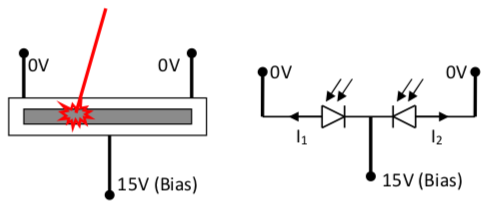
\includegraphics[width=0.75\textwidth]{images/GrundlagenLaserentfernungsmessung/PSD}
	\caption{Aufbau einer \ac{PSD} \cite{APD_Scematic}}
\end{figure}
Wenn man nun jeweils den Photostrom der Dioden miteinander Vergleicht kann man eine sehr präzise Auskunft über die Position des Lichtpunkts geben.
\begin{equation}\formelentry{Position des Lichtpunkts einer \ac{PSD}}
	x = \frac{I_1 - I_2}{I_1 + I_2}
\end{equation}
\begin{flalign*}
	&I_1 = \text{Strom aus der linken Photodiode}\left[A \right]&\\
	&I_2 = \text{Strom aus der rechten Photodiode} \left[A \right]&\\
	&x = \text{Relative Position des Lichtpunktes}&
\end{flalign*}
Die Differenz der Ströme wird hier auf den Gesamtstrom Normiert, dies hat zur Folge, dass die Position unabhängig von der Intensität des Lichts wird.\\
Um diese Auswertung zu realisieren ist lediglich eine Transimpedanzverstärkerschaltung gekoppelt mit einer Komperatorschaltung nötig, mit welcher die Spannungen verglichen werden können.\\
Ein sehr großer Vorteil der \ac{PSD} gegenüber anderer Methoden zur Feststellung der Position eines Lichtpunkts ist, dass die \ac{PSD} innerhalb von Nanosekunden reagieren und das mit einer Sehr genauen Auflösung.\cite{psd}

